\documentclass[
	t, % align text inside frame to t=top, b=bottom, c=center
	10pt, % 8pt, 9pt, 10pt, 11pt, 12pt, 14pt, 17pt, 20pt available as text font
	aspectratio=1610, % select your aspect ratio 4:3=43, 16:9=169, 16:10=1610
	ngerman,
	english,
	%handout,
	]{beamer}
\usetheme{Juelich}

\usepackage{babel}
\usepackage[utf8]{inputenc}
\usepackage{tikz}
\usepackage{listings}
\usepackage{xpatch}
\usepackage{minted}
\usepackage{pgf}
\usepackage{hyperref}

\usepackage{svg}

\def\figpath{figures/}
\def\width{16.4} % slide width
\def\height{8.5} % slide height
\newcommand{\showgrid}{%
  \pgfsetlinewidth{0.8pt}
  \pgfgrid[step={\pgfpoint{1cm}{1cm}}]{\pgforigin}{\pgfxy(\width,\height)}{}
  \pgfsetlinewidth{0.1pt}
  \pgfgrid[stepx=0.1cm,stepy=0.1cm]{\pgforigin}{\pgfxy(\width,\height)}
}
\newcommand{\pgfslide}[1]{
  \hspace*{-1cm}
  \begin{pgfpicture}{0cm}{0cm}{\width cm}{\height cm}
    #1
  \end{pgfpicture}
}


\title{\Large Part 1: Introduction to NEST}
\subtitle{\large Introduction to the simulation of structurally detailed large-scale neuronal networks}
\author{Alexander van Meegen, Dennis Terhorst}
\institute{INM-6, IAS-6, INM-10; J{\"u}lich Research Centre}
\date{13 July 2019}
\titlegraphic{\includegraphics
	[height=0.2\paperheight]{\figpath nest-and-snakemake.png}
}


\begin{document}

\definecolor{goodgreen}{rgb}{0,0.81,0.04001}
\definecolor{goodred}{rgb}{0.91,0,0.04001}
\newcommand{\pro}{\textbf{\color{goodgreen}+}}
\newcommand{\con}{\textbf{\color{goodred}--}}

\fzjset{title page=image}
\maketitle

\def\ttl{Multi-scale brain structure and dynamics}
\section{\ttl}
\begin{frame}
  \frametitle{\ttl}
  \pgfslide{
    \pgfputat{\pgfxy(8.0,4.75)}{
      \def\picname{scales.pdf}
      \pgfdeclareimage[interpolate=true,width=7.5cm]{\picname}{\figpath\picname}
      \pgfbox[center,center]{\pgfuseimage{\picname}}
    }
    \pgfputat{\pgfxy(8.8,1.)}{\pgfbox[left,top]{\parbox{7.0cm}{\centering
      \tiny [Dahmen, 2017]
    }}}
    %\showgrid
  }
\end{frame}


\def\ttl{The microcircuit model}
\section{\ttl}
\begin{frame}
  \frametitle{\ttl}
  \pgfslide{

    \pgfputat{\pgfxy(0.8,8.3)}{\pgfbox[left,top]{\parbox{7.0cm}{\centering
      \begin{itemize}
        \item $10^5$ identical leaky-integrate and fire neurons
        \item $3\cdot10^8$ exponentially decaying synaptic currents
        \item four layers with one excitatory and one inhibitory population each
        \item size of populations and connection probabilities deduced from anatomical data sets % for example electrophysiological recordings
      \end{itemize}
      }}}
    \pgfputat{\pgfxy(0.8,3.5)}{\pgfbox[left,top]{\parbox{12.0cm}{\centering
      \begin{itemize}
        \item asynchronous irregular and cell-type specific firing rates
        \item thalamic stimulation elicits flow of activity through cortical layers
      \end{itemize}
      }}}

    \pgfputat{\pgfxy(10.0,6.0)}{
      \def\picname{column.pdf}
      \pgfdeclareimage[interpolate=true,width=3.0cm]{\picname}{\figpath\picname}
      \pgfbox[center,center]{\pgfuseimage{\picname}}
     }

    \pgfputat{\pgfxy(0.8,2.2)}{\pgfbox[left,top]{\parbox{12.0cm}{\centering
      \flushleft\footnotesize Potjans and Diesmann (2014) The Cell-Type Specific Cortical Microcircuit: Relating Structure and Activity in a Full-Scale Spiking Network Model. Cerebral Cortex 24(3):785-806
      }}}
  }
\end{frame}


\def\ttl{The multi-area model}
\section{\ttl}
\begin{frame}
  \frametitle{\ttl}
  \pgfslide{

    \pgfputat{\pgfxy(0.8,8.3)}{\pgfbox[left,top]{\parbox{5.0cm}{\centering
      \begin{itemize}
        \item<1-> full-density model of macaque visual cortex
        \item axonal tracing data from the CoCoMac database, which are systematically refined using dynamical constraints
        \item stable asynchronous irregular ground state
      \end{itemize}
      }}}
    \pgfputat{\pgfxy(0.8,3.8)}{\pgfbox[left,top]{\parbox{12.0cm}{\centering
      \begin{itemize}
        \item produces realistic spiking statistics in V1
        \item functional connectivity compares to fMRI measurements
      \end{itemize}
      }}}

    \pgfputat{\pgfxy(9.65,6.5)}{
      \def\picname{MAM.pdf}
      \pgfdeclareimage[interpolate=true,width=7.0cm]{\picname}{\figpath\picname}
      \pgfbox[center,center]{\pgfuseimage{\picname}}
     }

    \pgfputat{\pgfxy(0.8,2.6)}{\pgfbox[left,top]{\parbox{12.0cm}{\centering
      \flushleft\footnotesize Schmidt et al. (2018) Multi-scale account of the network structure of macaque visual cortex. Brain Structure and Function 223(3):1409-1435\\
      Schmidt et al. (2018) A multi-scale layer-resolved spiking network model of resting-state dynamics in macaque visual cortical areas. PLOS CB 14(10):e1006359
      }}}
  }
\end{frame}


\def\ttl{Importance of the correct network size}
\section{\ttl}
\begin{frame}
  \frametitle{\ttl}
  \pgfslide{

    \pgfputat{\pgfxy(0.8,8.3)}{\pgfbox[left,top]{\parbox{5.0cm}{\centering
          \begin{itemize}
              \item<1-> under which conditions can a small network represent a subsampled larger network?
              \item analyzes scalability of binary and LIF neuron networks
          \end{itemize}
        }}}
    \pgfputat{\pgfxy(0.8,4.3)}{\pgfbox[left,top]{\parbox{12.0cm}{\centering
          \begin{itemize}
              \item mean activity can be preserved by adjusting the mean and variance of the input
              \item temporal structure of pairwise averaged correlations depends on the effective connectivity and cannot always be preserved
          \end{itemize}
        }}}
    \pgfputat{\pgfxy(9.5,6.5)}{
      \def\picname{Albada2015.pdf}
      \pgfdeclareimage[interpolate=true,width=6.5cm]{\picname}{\figpath\picname}
      \pgfbox[center,center]{\pgfuseimage{\picname}}
     }

    \pgfputat{\pgfxy(0.8,2.2)}{\pgfbox[left,top]{\parbox{12.0cm}{\centering
      \flushleft\footnotesize van Albada et al. (2015) Scalability of Asynchronous Networks Is Limited by One-to-One Mapping between Effective Connectivity and Correlations. PLOS CB 11(9):e1004490
      }}}
  }
\end{frame}


\def\ttl{NEST = NEural Simulation Tool}
\section{\ttl}
\begin{frame}
  \frametitle{\ttl}
  \pgfslide{
    \pgfputat{\pgfxy(0.8,8.3)}{\pgfbox[left,top]{\parbox{12.0cm}{\centering
          \begin{itemize}
              \item<1-> Focus on the dynamics, size and structure of neural systems rather than on the exact morphology of individual neurons
              \item<1-> NEST runs on laptops ({\footnotesize{Linux, Mac OS X ($\geq$10.3), Windows via virtualization}}) as well as supercomputers $\rightarrow$ simulations of large-scale models
              \item<1-> NEST is a hybrid parallel (OpenMP+MPI) simulator for spiking neural networks, written in C++ with a Python front end
          \end{itemize}
        }}}

    \pgfputat{\pgfxy(0.8,4.0)}{\pgfbox[left,top]{\parbox{6.0cm}{\centering
          \begin{itemize}
              \item<1-> Get publication and source code on http://nest-simulator.org
          \end{itemize}
        }}}

\pgfputat{\pgfxy(9.5,3.)}{
      \def\picname{K.pdf}
      \pgfdeclareimage[interpolate=true,width=5cm]{\picname}{\figpath\picname}
      \pgfbox[center,center]{\pgfuseimage{\picname}}
     }
  }
\end{frame}


\def\ttl{Programming languages}
\section{\ttl}
\begin{frame}
  \frametitle{\ttl}
  \pgfslide{
    \pgfputat{\pgfxy(0.8,8.3)}{\pgfbox[left,top]{\parbox{6.cm}{\centering
          \begin{itemize}
            \item C++ kernel
            \item Built-in simulation language interpreter (SLI)
            \item Python-based user interface (PyNEST)
          \end{itemize}
        }}}
    \pgfputat{\pgfxy(0.8,4.3)}{\pgfbox[left,top]{\parbox{6.cm}{\centering
          \begin{itemize}
            \item Back end for the simulator- independent modeling tool PyNN
            \item Interface to the Multi Simulator Coordinator MUSIC
          \end{itemize}
        }}}


    \pgfputat{\pgfxy(10.0,5.0)}{
      \begin{pgfrotateby}{\pgfdegree{270}}
      \def\picname{python_interface.pdf}
      \pgfdeclareimage[interpolate=true,width=6cm]{\picname}{\figpath\picname}
      \pgfbox[center,center]{\pgfuseimage{\picname}}
      \end{pgfrotateby}
     }
     }
\end{frame}


\def\ttl{Three main components of a NEST simulation}
\section{\ttl}
\begin{frame}
  \frametitle{\ttl}
  \pgfslide{
    \pgfputat{\pgfxy(0.8,8.3)}{\pgfbox[left,top]{\parbox{12.0cm}{\centering
\begin{itemize}
\item \textbf{Nodes}
\begin{itemize}
	\item Neurons -- Devices (-- Sub-networks)
	\item Have dynamic state variable(s) that changes over time ($V_\mathrm{m}(t)$)
	\item Can be affected by events (spikes)
	\end{itemize}
\item \textbf{Events}
	\begin{itemize}
	\item Pieces of information of a particular type
	(e.g., spike, voltage or current event)
	\item Recording devices: \url{`spike_detector', `voltmeter', `multimeter'}
	\end{itemize}
\item \textbf{Connections}
	\begin{itemize}
	\item Communication channels for the exchange of events
	\item Directed (from source node to target node)
	\item Weighted (how strongly does an event influence the target node)
	\item Delayed (length of transmission duration between source and target)
	\item Connections are created using one global \url{Connect} function
	\end{itemize}
\end{itemize}
}}}
}
\end{frame}


\def\ttl{NEST neuron and synapse models}
\section{\ttl}
\begin{frame}
  \frametitle{\ttl}
  \pgfslide{
    \pgfputat{\pgfxy(6.7,4.7)}{
      \def\picname{models.pdf}
      \pgfdeclareimage[interpolate=true,width=12.3cm]{\picname}{\figpath\picname}
      \pgfbox[center,center]{\pgfuseimage{\picname}}
     }
  }
\end{frame}

\def\ttl{Event-driven vs.~time-driven simulation}
\section{\ttl}
\begin{frame}
  \frametitle{\ttl}
  \pgfslide{
    \pgfputat{\pgfxy(0.6,7.8)}{\pgfbox[left,top]{\parbox{11.5cm}{
          \begin{tabular}{p{1cm}|p{5cm}|p{5.3cm}}
            & \bf Event-driven & \bf Time-driven\\[1ex]
            \hline\vspace*{1ex}
            {\bf Pros}
            &%
            \begin{itemize}
            \item more efficient for low input rates
            \item `correct' solution for invertible neuron models
            \end{itemize}
            &%
            \begin{itemize}
            \item more efficient for high input rates
            \item works for all neuron models
            \item scales well
            \end{itemize}
            \\
            \hline\vspace*{1ex}
            {\bf Cons}
            &%
            \begin{itemize}
            \item only works for neurons with invertible dynamics
            \item event queue does not scale well
            \end{itemize}
            &%
            \begin{itemize}
            \item only `approximate' solution even for analytically solvable models
            \item spikes can be missed due to discrete sampling of membrane potential
            \end{itemize}
          \end{tabular}
     }}}
  %%
  %%\showgrid
  }
\end{frame}


\def\ttl{Event-driven vs.~time-driven simulation}
\begin{frame}
  \frametitle{\ttl}
  \pgfslide{
    \pgfputat{\pgfxy(0.8,8.5)}{\pgfbox[left,top]{\parbox{12.0cm}{\centering
   \flushleft NEST: hybrid approach to simulation
                \begin{itemize}
                \item input events to neurons are frequent: time-driven algorithm
                  \begin{itemize}
          \item If the dynamics is nonlinear, we need a numerical method to solve it,
            e.g.:
            \begin{itemize}
            \item Forward Euler: \quad $y([i+1]h)=y(ih)+h\cdot\dot{y}(ih)$
            \item Runge-Kutta ($k$th order)
            \item Runge-Kutte-Fehlberg with adaptive step size
            \item \ldots
            \end{itemize}
           \item<1->[$\rightarrow$]
             Use a pre-implemented solver, for example, from the GNU Scientific Library (GSL).
             \\[2ex]
           \item<1->
             \alert{If the dynamics is linear (e.g.~LIF or MAT), we can solve it exactly.}
       \end{itemize}
                \item events at synapses are rare: event driven component
                  \begin{itemize}
                  \item Exception: gap junctions
                  \end{itemize}
                \end{itemize}
        }}}
  }
\end{frame}


\def\ttl{Exact integration of linear time-invariant systems}
\section{\ttl}
\begin{frame}
  \frametitle{\ttl}
  \pgfslide{
    \only{
      \pgfputat{\pgfxy(6.2,4.1)}{
        \def\picname{Rotter99a_prop.pdf}
        \pgfdeclareimage[interpolate=true,width=6cm]{\picname}{\figpath\picname}
        \pgfbox[center,center]{\pgfuseimage{\picname}}
      }
    }
    \pgfputat{\pgfxy(0.8,8.3)}{\pgfbox[left,top]{\parbox{12.cm}{
          \begin{itemize}
          \item consider time-invariant linear system
            \begin{math}
              \alert{\dot{y}=Ay+x}
            \end{math}\\
          \item[$\rightarrow$] \alert{exact} solution:
            \begin{math}\displaystyle
              y(t)=e^{A(t-s)}y(s)+\int_{s_+}^{t} e^{A(t-\tau)}x(\tau)\,d\tau
            \end{math}\\
          \item time grid: $\{t_k=k\cdot{}h\,|\,k=1,2,\ldots\}$;
                    spike train:
            \begin{math}\displaystyle
              x(t)=\sum_k x_k\delta(t-t_k)
            \end{math}
          \item [$\rightarrow$] general solution:
            \begin{math}\displaystyle
              \alert{y_{k+1}=e^{Ah}y_k+x_{k+1}}
            \end{math}
            % integral turns into sum -> iteration, y_k is propagated and x_k+1 is added
          \item iterative propagation of solution\\[8ex]
          \item[] with  \alert{propagator} (matrix) $P(h)=e^{Ah}$
       \end{itemize}
     }}}

     \pgfputat{\pgfxy(0.8,2.2)}{\pgfbox[left,top]{\parbox{12.0cm}{\centering
       \flushleft\footnotesize Rotter and Diesmann (1999)
       Exact digital simulation of time-invariant linear systems with applications to neuronal modeling.
       Biological Cybernetics 81(5-6):381-402
     }}}
  %%\showgrid
  }
\end{frame}


\def\ttl{Representation of network structure: serial}
\section{\ttl}
\begin{frame}
  \frametitle{\ttl}
  \pgfslide{
    \pgfputat{\pgfxy(0.8,3.5)}{\pgfbox[left,top]{\parbox{12.5cm}{\centering
          \begin{itemize}
          \item<1-> each neuron and synapse maintains its own parameters
          \item synapses save the index of the target neuron
          \end{itemize}
        }}}
    \pgfputat{\pgfxy(7.0,6.)}{
      \def\picname{network_representation_serial.pdf}
      \pgfdeclareimage[interpolate=true,width=8cm]{\picname}{\figpath\picname}
      \pgfbox[center,center]{\pgfuseimage{\picname}}
     }

    %% \showgrid
  }
\end{frame}


\def\ttl{Representation of network structure: distributed}
\section{\ttl}
\begin{frame}
  \frametitle{\ttl}
  \pgfslide{
    \pgfputat{\pgfxy(0.8,8.2)}{\pgfbox[left,top]{\parbox{6.cm}{\centering
          \begin{itemize}
          \item modulo operation distributes neurons
          \item one target list for every neuron on each machine
          \item synapse stored on machine that hosts the target neuron
          \item connections are established on each machine and the connectivity information subsequently propagated to other machines
            \begin{itemize}
              \item[$\rightarrow$] wiring is a parallelizable task
          \end{itemize}
          \end{itemize}
        }}}
    \pgfputat{\pgfxy(10.0,4.8)}{
      \def\picname{network_dist.pdf}
      \pgfdeclareimage[interpolate=true,width=5.2cm]{\picname}{\figpath\picname}
      \pgfbox[center,center]{\pgfuseimage{\picname}}
     }
    %% \showgrid
  }
\end{frame}


\def\ttl{Creating custom models}
\section{\ttl}
\begin{frame}
  \frametitle{\ttl}
  \pgfslide{
    \pgfputat{\pgfxy(0.8,8.2)}{\pgfbox[left,top]{\parbox{12.6cm}{\centering
          \begin{itemize}
          \item Discuss with developers via user mailing list
            \begin{itemize}
              \item if your idea makes sense
              \item if it has not yet been implemented
            \end{itemize}
          \item Only create models for NEST versions $>$ 2.10
            \begin{itemize}
              \item Start from most similar existing model
              \item It may end up in a release!
            \end{itemize}
          \end{itemize}
          %\vspace*{5mm}
          \begin{itemize}
          \item {\bf NESTML (NEST Modeling Language)}
            \begin{itemize}
            \item New simplified language with syntax similar to Python (recommended)
            \item \footnotesize{\url{https://github.com/nest/nestml}}
            \item Currently enables developing neuron but not yet synapse models
            %\item Plotnikov et al. "NESTML: a modeling language for spiking neurons" arXiv:1606.02882 (2016).
            \end{itemize}
          \item Extension modules (C++)
            \begin{itemize}
            \item loaded dynamically
            \item \footnotesize{\url{http://nest.github.io/nest-simulator/extension_modules}}
            %\item Start from examples/MyModule
            %\item Load module: nest.Install("mymodule")
            %\item Details are about to change
            \end{itemize}
          \item Inside NEST (C++)
            %\begin{itemize}
            %\item No need to load separately
            %\item Allows others to use your code
            %\end{itemize}
          \end{itemize}
        }}}
  }
\end{frame}


\def\ttl{Topology}
\section{\ttl}
\begin{frame}[fragile]
  \frametitle{\ttl}
  \pgfslide{
    \pgfputat{\pgfxy(16,9.0)}{\pgfbox[right,top]{
      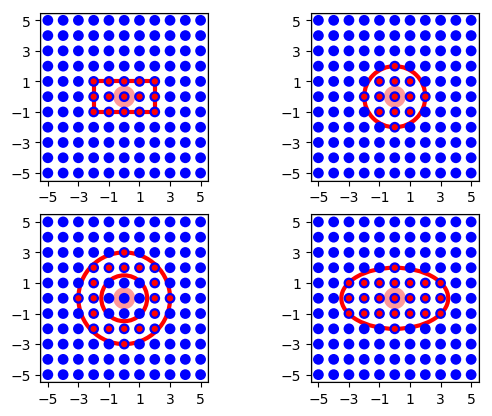
\includegraphics[width=5cm]{figures/conn2_a}}
    }
    \pgfputat{\pgfxy(16,4.8)}{\pgfbox[right,top]{
      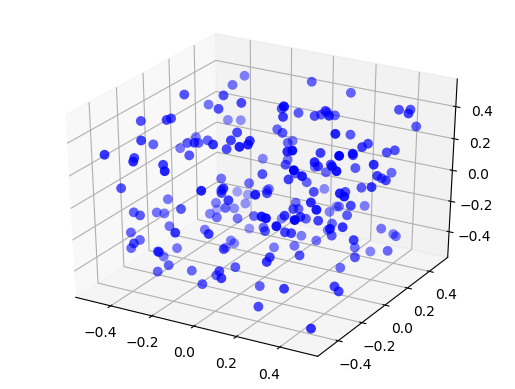
\includegraphics[width=5cm]{figures/layer4_3d}}
    }
    \pgfputat{\pgfxy(0.8,8.0)}{\pgfbox[left,top]{
      \parbox{.6\textwidth}{\centering


      \begin{itemize}
      \item Functionality
        \begin{itemize}
        \item Lay out elements on grids or at arbitrary points in space (2D or 3D)
        \item Elements can be neurons or combinations of neurons and devices
        \item Connect neurons in a position- and distance-dependent manner
        \item Set periodic boundary conditions
        \item Choose whether to allow self-connections (autapses) or multiple connections (multapses)
        \item Distance-dependent or random weights and delays
        \end{itemize}
      \item
        User manual: \url{https://www.nest-simulator.org/documentation} $\to$ Topology
      \end{itemize}
    }}}
  }
\end{frame}


\def\ttl{Why should I use NEST?}
\section{\ttl}
\begin{frame}[fragile]
  \frametitle{\ttl}
  \pgfslide{
    \pgfputat{\pgfxy(0.8,8.0)}{\pgfbox[left,top]{\parbox{12.cm}{\centering
      \begin{enumerate}
      \item NEST provides over 50 neuron models
      \item NEST provides over 10 synapse models, including short-term plasticity (Tsodyks \& Markram)
      and different variants of STDP
      \item NEST provides many examples that help you getting started % with your own simulation project
      % \item NEST offers convenient and efficient commands to define and connect large networks,
      % ranging from algorithmically determined connections to data-driven connectivity
      \item NEST lets you inspect and modify the state of each neuron and each connection at any time during a simulation
      \item NEST is fast and memory efficient; it makes best use of your multi-core computer and compute clusters %with minimal user intervention
      \item NEST has a large and experienced developer community %of all neural simulators
      \item NEST was first released in 1994 under the name SYNOD and has been extended and improved ever since
      \item NEST is open source software and is licensed under the GPL 2
    \end{enumerate}
    }}}
  }
\end{frame}


\def\ttl{Anaconda, Miniconda, ...}
\section{\ttl}
\begin{frame}[fragile]
  \frametitle{\ttl}

  \begin{flushright}
  \raisebox{0pt}[0pt]{
  \includesvg[pretex=\tiny,svgpath={figures/}, width=.3\textwidth]{conda_logo}}
  \end{flushright}
  User space package management system
  \begin{itemize}
  \item[\pro] isolates installations of different packages
  \item[\pro] includes system libraries (in contrast language specific managers like pip)
  \item[\pro] can export environment definition
  \item[\con] interactions with base environment / system \& language package managers
  \item[\con] requires basic understanding of bash environment (\lstinline[language=bash]{$PATH}, \lstinline[language=bash]{$PYTHONPATH}, \lstinline[language=bash]{$LD_LIBRARY_PATH}, \ldots)
  \item[\con] non-trivial dependency management
  \end{itemize}

  \vspace*{.2cm}
  {\large Installation}
  \begin{enumerate}
  \item Download \url{https://docs.conda.io/en/latest/miniconda.html},\\\hspace*{1cm}(probably Miniconda3, 64-bit)
  \item open new terminal window
  \end{enumerate}

\end{frame}


\def\ttl{Installation (conda)}
\section{\ttl}
\begin{frame}[fragile]
  \frametitle{\ttl}

  \begin{lstlisting}
   conda env create --file environment.yml
  \end{lstlisting}
  with \lstinline{environment.yml} defining the package environment
  \hspace*{3.7cm}\parbox{.7\textwidth}{
  \lstinputlisting{../../environment.yml}
  }
\end{frame}


\def\ttl{Installation (apt, experimental)}
\section{\ttl}
\begin{frame}[fragile]
  \frametitle{\ttl}

    Add a personal package archive to find NEST package:
    \begin{lstlisting}
    sudo add-apt-repository ppa:nest-simulator/nest
    sudo apt-get update
    sudo apt-get install nest
    \end{lstlisting}

    After the installation:
    \begin{lstlisting}
    source /usr/bin/nest_vars.sh
    \end{lstlisting}
    or add this line to your \lstinline{.bashrc}.

    NEST was built with '-Dwith-python=3' and is installed to \lstinline{/usr}!
    Python 2 will not know anything.
\end{frame}


\def\ttl{Now hands-on}
\section{\ttl}
\begin{frame}[fragile]
  \frametitle{\ttl}
	\pgfslide{
	      \pgfputat{\pgfxy(0.8,8.2)}{\pgfbox[left,top]{\parbox{12.cm}{\centering
	          \begin{enumerate}
	          \item{\bf Install NEST}
							\begin{itemize}
								\item Instructions: \url{https://www.nest-simulator.org/documentation/}
								\item On Windows use a virtual machine (USB sticks with image available)
								\item On Ubuntu you can also use a PPA: \url{ppa:nest-simulator/nest}
							\end{itemize}
	          \item{\bf Get the exercises}
						\begin{itemize}
							\item Go to \url{https://github.com/alexvanmeegen/CNS2019_NEST_Tutorial}
							\item Download as zip (or clone)
						\end{itemize}
						\item{\bf Enjoy the ride}
							\begin{itemize}
								\item Open \url{0_hello_world.ipynb} for a first glance
								\item Get going with \url{1_first_steps.ipynb}
							\end{itemize}
	          \end{enumerate}
	    }}}
	}
\end{frame}

\def\ttl{Background}
\section{\ttl}
\begin{frame}[fragile]
  \vspace*{.45\textheight}
  \begin{center}
  {\Large \textbf{\ttl}}
  \end{center}
\end{frame}

\def\ttl{Conda Dependencies...}
\section{\ttl}
\begin{frame}[fragile]
  \frametitle{\ttl}

  \begin{lstlisting}
   conda create -n nest-tutorial
   conda activate nest-tutorial
   conda install jupyter
   conda install -c conda-forge nest-simulator
   ...
  \end{lstlisting}
  \begin{center}
   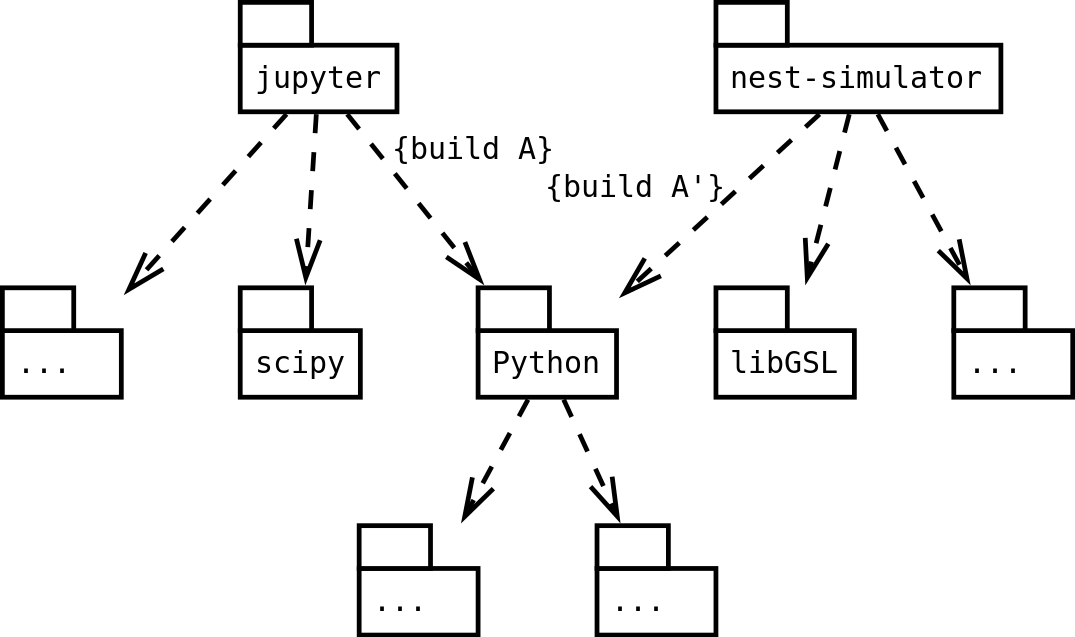
\includegraphics[height=.4\textheight]{figures/conda-dependency-management.png}

  \vspace*{.2cm}$\Rightarrow$ replacing Python makes Jupyther loose it's kernel!
  \end{center}
\end{frame}


\end{document}
